\documentclass[ngerman]{beamer}
\usepackage{babel}
\usepackage[latin1]{inputenc}
\usepackage[T1]{fontenc}
\usepackage{lmodern}
\usepackage{graphicx}

    \usetheme{TUC2}
%    \usefonttheme{structureitalicserif}
    \setbeamercovered{transparent}

\mode<presentation>
    \title{Amazon EC2}
    \subtitle{EC2 virtual server und EC2 container}
    \author{Christian Rebischke}
    \institute{Institut f�r Informatik}
    \date{2017-07-04}


%%%%%%%%%%%%%%%%%%%%%%%%%%%%%%%%%%%%%%%%%%%%%%%%%%%%%%
\begin{document}
\begin{frame}
\titlepage
\end{frame}

\begin{frame}
\frametitle{Agenda}
\tableofcontents
\end{frame}
%%%%%%%%%%%%%%%%%%%%%%%%%%%%%%%%%%%%%%%%%%%%%%%%%%%%%%

\section{Einf�hrung in Amazon EC2}
\begin{frame}
    \frametitle{Warum Amazon EC2?}
    \begin{itemize}
        \item Flexible Kosten
        \item Weltweite Infrastruktur
        \item Software as a Service
        \item Einfache Skalierung
        \item Server on Demand
    \end{itemize}
\end{frame}

\begin{frame}
    \frametitle{Vertikale vs Horizontale Skalierung}
    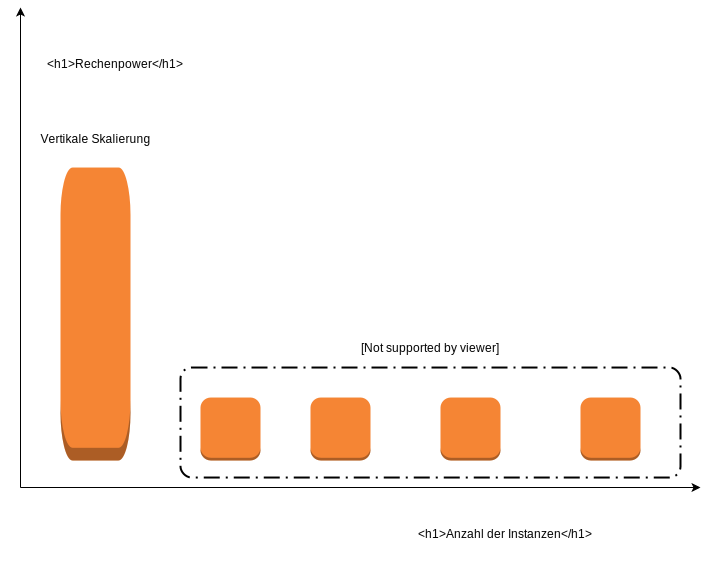
\includegraphics[width=1.0\textwidth]{figures/scalability.pdf}
\end{frame}

\begin{frame}
    \frametitle{Begrifflichkeiten}
    \begin{itemize}
        \item Amazon Machine Image (AMI)
        \item Instance Type
    \end{itemize}
    \includegraphics[width=0.5\textwidth]{figures/instance.pdf}
\end{frame}

\begin{frame}
    \frametitle{}
\end{frame}

\section{Regionen}
\section{Virtualisierungstechnik}
\section{EC2 Container}
\section{Sicherheit}


\end{document}
